\documentclass[b5paper,widemargins,twoside,printrev]{jb-thesis}
\usepackage[T1]{fontenc}
\usepackage[charter, uppercase=upright]{mathdesign}
\usepackage[semibold,type1]{sourcesanspro}
\usepackage{amsmath, amsthm}
\usepackage{mathtools}
\usepackage{algorithm2e}
\usepackage{color}
\usepackage{upgreek}
\usepackage{graphicx, xcolor}
\usepackage{tikzpagenodes}
\usepackage{cleveref}
\usepackage{blindtext}

%%%%%%%%%%%%

% Package-dependent commands
\newtheorem{theorem}{Theorem}[section]
\newtheorem{definition}{Definition}[section]
\newtheorem{lemma}[theorem]{Lemma}
\newtheorem{proposition}[theorem]{Proposition}
\newtheorem{corollary}[theorem]{Corollary}

%algorithms adjustments
\SetAlFnt{\sffamily}
\newcommand{\sftmp}[1]{\sffamily\textbf{#1}}
\SetKwSty{sftmp}
\SetArgSty{sftmp}

%cleveref adjustments
\crefname{algocf}{alg.}{algs.}
\Crefname{algocf}{Algorithm}{Algorithms}

% bullet not available in italic -- always use math version
\renewcommand\textbullet{\ensuremath{\bullet}}

%%%%%%%%%%%%
% Editing commands
\newcommand{\todo}[1]{{\color{red} TODO: #1}}
\newcommand{\note}[1]{{\color{blue} NOTE: #1}}
\newcommand{\hide}[1]{}

% Abbreviations
\newcommand{\mnist}{{\sc MNIST} }
\newcommand{\tidigits}{{\sc TIDIGITS} }
\newcommand{\adam}{{\sc ADAM} }

% Subplot labels
\newcommand{\spl}[1]{\textsf{\textbf{#1}}}

% Punctuation inside quotes
\newcommand{\qcomma}{\makebox[0pt][l]{,}}
\newcommand{\qpoint}{\makebox[0pt][l]{,}}


%%%%%%%%%%%%
% Mathbf symbols, expanded for simplicity
\newcommand{\ba}{\mathbf{a}}
\newcommand{\bb}{\mathbf{b}}
\newcommand{\bc}{\mathbf{c}}
\newcommand{\bd}{\mathbf{d}}
\newcommand{\be}{\mathbf{e}}
%\newcommand{\bf}{\mathbf{f}} \bf is defined already
\newcommand{\bg}{\mathbf{g}}
\newcommand{\bh}{\mathbf{h}}
\newcommand{\bi}{\mathbf{i}}
\newcommand{\bj}{\mathbf{j}}
\newcommand{\bk}{\mathbf{k}}
\newcommand{\bl}{\mathbf{l}}
\newcommand{\bm}{\mathbf{m}}
\newcommand{\bn}{\mathbf{n}}
\newcommand{\bo}{\mathbf{o}}
\newcommand{\bp}{\mathbf{p}}
\newcommand{\bq}{\mathbf{q}}
\newcommand{\br}{\mathbf{r}}
\newcommand{\bs}{\mathbf{s}}
\newcommand{\bt}{\mathbf{t}}
\newcommand{\bu}{\mathbf{u}}
\newcommand{\bv}{\mathbf{v}}
\newcommand{\bw}{\mathbf{w}}
\newcommand{\bx}{\mathbf{x}}
\newcommand{\by}{\mathbf{y}}
\newcommand{\bz}{\mathbf{z}}
\newcommand{\bA}{\mathbf{A}}
\newcommand{\bB}{\mathbf{B}}
\newcommand{\bC}{\mathbf{C}}
\newcommand{\bD}{\mathbf{D}}
\newcommand{\bE}{\mathbf{E}}
\newcommand{\bF}{\mathbf{F}}
\newcommand{\bG}{\mathbf{G}}
\newcommand{\bH}{\mathbf{H}}
\newcommand{\bI}{\mathbf{I}}
\newcommand{\bJ}{\mathbf{J}}
\newcommand{\bK}{\mathbf{K}}
\newcommand{\bL}{\mathbf{L}}
\newcommand{\bM}{\mathbf{M}}
\newcommand{\bN}{\mathbf{N}}
\newcommand{\bO}{\mathbf{O}}
\newcommand{\bP}{\mathbf{P}}
\newcommand{\bQ}{\mathbf{Q}}
\newcommand{\bR}{\mathbf{R}}
\newcommand{\bS}{\mathbf{S}}
\newcommand{\bT}{\mathbf{T}}
\newcommand{\bU}{\mathbf{U}}
\newcommand{\bV}{\mathbf{V}}
\newcommand{\bW}{\mathbf{W}}
\newcommand{\bX}{\mathbf{X}}
\newcommand{\bY}{\mathbf{Y}}
\newcommand{\bZ}{\mathbf{Z}}
% Greek symbols
\newcommand{\bdelta}{\boldsymbol{\delta}}
\newcommand{\bzeta}{\boldsymbol{\zeta}}
\newcommand{\btheta}{\boldsymbol{\theta}}
\newcommand{\bpi}{\boldsymbol{\pi}}
\newcommand{\bxi}{\boldsymbol{\xi}}
\newcommand{\bphi}{\boldsymbol{\phi}}
\newcommand{\bPhi}{\boldsymbol{\Phi}}
\newcommand{\bmu}{\boldsymbol{\mu}}
\newcommand{\bTheta}{\boldsymbol{\Theta}}
\newcommand{\bSigma}{\boldsymbol{\Sigma}}
\newcommand{\bGamma}{\boldsymbol{\Gamma}}
\newcommand{\bgamma}{\boldsymbol{\gamma}}
\newcommand{\bbeta}{\boldsymbol{\beta}}
\newcommand{\bomega}{\boldsymbol{\omega}}
\newcommand{\bpsi}{\boldsymbol{\psi}}
\newcommand{\blambda}{\boldsymbol{\lambda}}
\newcommand{\bLambda}{\boldsymbol{\Lambda}}
\newcommand{\bkappa}{\boldsymbol{\kappa}}
\newcommand{\btau}{\boldsymbol{\tau}}
\newcommand{\balpha}{\boldsymbol{\alpha}}

% Common function names
\newcommand{\Var}{\text{Var}}
\newcommand{\Dir}{\text{Dir}}
\newcommand{\Multi}{\text{Multi}}

% Common operations
\newcommand{\argmin}[1]{\underset{#1}{\mathrm{argmin}} \:}
\newcommand{\argmax}[1]{\underset{#1}{\mathrm{argmax}} \:}
\newcommand{\pd}[2]{\frac{\partial #1}{\partial #2}}



% biblatex
\usepackage[
    refsection=part,
    natbib,
    style=nature,
    citestyle=authoryear-comp,
    backend=biber,
    uniquename=false,
]{biblatex}

% adjust citation and bibliography commands
\preto\fullcite{\AtNextCite{\defcounter{maxnames}{99}}}
\defbibheading{bibliography}[\bibname]{%
    \chapter*{#1}%
    \addcontentsline{toc}{chapter}{\numberline{}#1}%
    \markboth{#1}{#1}
}
\addbibresource{bibliography.bib}
\setcounter{tocdepth}{1}
%

% specify your details...
\degree{{\sc Doctor of Sciences} of ETH Zurich}
\degreeabbr{Dr. sc. ETH Zurich}
\gradyear{2017}

\author{Jonathan Binas}
\acadtitle{MSc. ETH Zurich}
\born{1/1/2017}
\citizen{La La Land}


\title{Brain-Inspired Models and Systems \\[0.7ex] for Distributed Computation}

\examiners{
    Prof. Dr. Abraham Bebraham \\
    Prof. Dr. X. Y. Zebraham
}

\date{\today}


% ---
\begin{document}

 \begin{preliminary}
    \maketitle
    \tableofcontents
    % \include{abstract}
 \end{preliminary}

 % you may or may not want to use parts to structure your thesis
 \part{Lorem Ipsum}

 % generate some random content...
 \blinddocument
 
 % the partextra command allows for arbitrary objects to be placed
 % on the part title page, here's an example:
 \setpartextra{
     \begin{tikzpicture}[remember picture, overlay]
	 \node[inner sep=0pt, yshift=-1.8in] at (current page text area) {
	     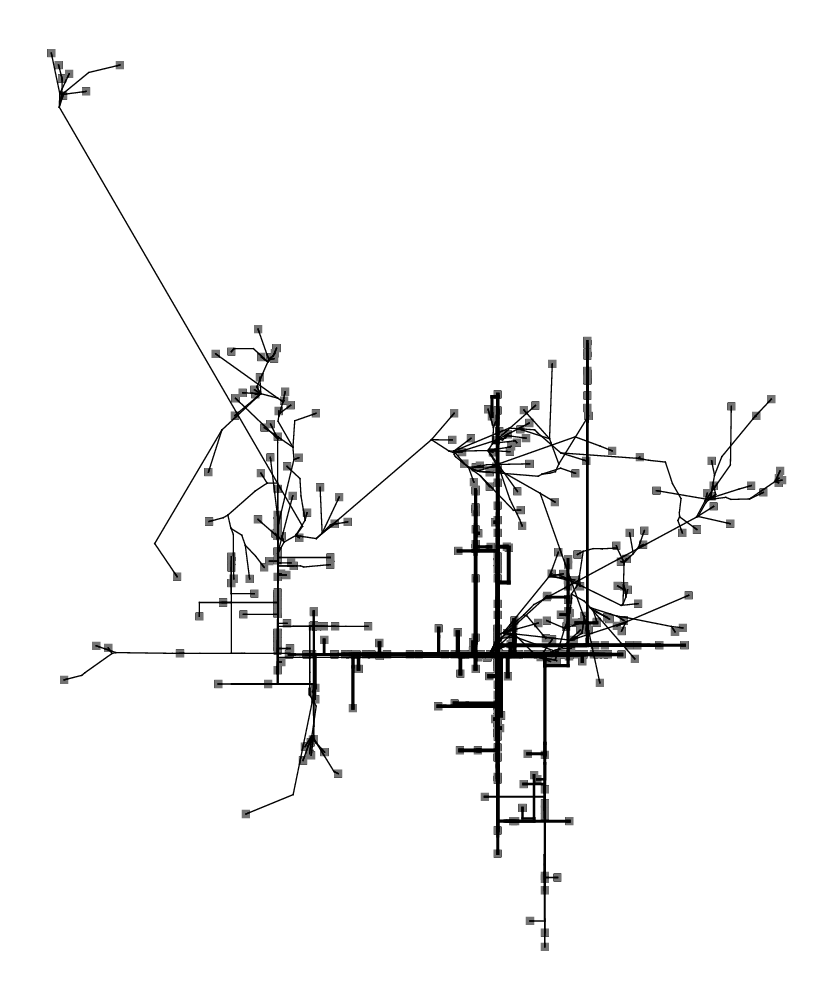
\includegraphics[scale=0.7]{neuron45c.png}};
     \end{tikzpicture}
 }

 % the partextra content will be applied to the subsequent part
 \part{Computing~with~imprecise and~noisy~substrates}

 % add an unnumbered section
 \mbox{}
 \section*{Introduction}

 Due to their organic nature, no two cells of a biological system, and therefore no two processing units of a brain, behave exactly the same.
 Signals are communicated electrically, chemically, on a molecular basis, and even mechanically, through the action of ion channels, whereby all of these processes are influenced by external factors, such as temperature, the abundance of various substances, and various sources of noise \citep{shadlen1994noise}.

 % let's add some math
 \section{Formal derivation}

 It is now easy to see that the state $\tilde{x}^\mathsf{b}$ corresponds to state $x^\mathsf{b}$ of the original model, since
 %
 \begin{align}
     \tilde{x}^\mathsf{b}_k &= \sigma\left(\sum_{j<k} w_{kj} x^\mathsf{f}_j + \sum_{j>k} \tilde{w}_{kj} (x^\mathsf{f}_j + \Delta x_j) + b_k\right) \\
	&=  \sigma\left(\sum_{j<k} w_{kj} x^\mathsf{f}_j + \sum_{j>k} \tilde{w}_{kj} x^\mathsf{b}_j + b_k\right) = x^\mathsf{b}_k\,.
     \label{eqn:random1}
 \end{align}
 %
 Analogously to the original derivation, it can be shown that the first and the second forward passes, as well as the subsequent backward pass do not increase the system energy.



 % print the bibliography
 \printbibliography


\end{document}


